% This is samplepaper.tex, a sample chapter demonstrating the
% LLNCS macro package for Springer Computer Science proceedings;
% Version 2.20 of 2017/10/04
%
\documentclass[runningheads]{llncs}
%
\usepackage{mwe}
\usepackage{graphicx}
\graphicspath{{figures/}}
\usepackage{color}
\definecolor{highlight}{rgb}{1,1,0.6}
\definecolor{link}{rgb}{0.5,0.0,0.0}
\definecolor{cite}{rgb}{0.0,0.0,0.6}
\definecolor{url} {rgb}{0.3,0.0,0.3}
\definecolor{grey}{rgb}{0.3,0.3,0.3}

\usepackage[hidelinks]{hyperref}
\hypersetup{
	colorlinks,
	linkcolor={cite},
	citecolor={cite},
	urlcolor ={cite}
}

\usepackage{tabularx}
\usepackage{array}
\usepackage{booktabs} % for nice rules/lines in tables
\usepackage{arydshln} % for dashed lines in tables

\usepackage{soul} % for highlighting text
\usepackage{xspace}
\usepackage[shortcuts]{extdash}
\usepackage{relsize} % used in the \anote and \comment macros.

%% annotation commands %% 
\newcommand{\anote}[1]{{\leavevmode\smaller\itshape\color{red}\{#1\}}}
\sethlcolor{highlight}
\newcommand{\comment}[2]{\hl{#1} {{\leavevmode\smaller\color{red}\itshape\{#2\}}}}

%% PM Define authornote command for comments
\newcommand{\authornote}[1] {
	\begin{center}
		\framebox{
			{\begin{minipage}[t]{0.9\linewidth}
					\raggedright  \textbf{[PM]}~ \scriptsize #1 \normalsize
			\end{minipage}}
		}
	\end{center}
}

\newcommand*{\bibfont}{\tiny}



\newcommand{\demon}{{DEMON}}
\newcommand{\infomap}{{Infomap}}

\usepackage{amssymb}
\usepackage{bm}
\usepackage{mathtools}

% custom commands
\usepackage{rotating}
\newcolumntype{P}[1]{>{\centering\arraybackslash}p{#1}}
\newcolumntype{Y}{>{\centering\arraybackslash}X}
\usepackage{subcaption}


\begin{document}
%
\title{Fantastic activists and how to find them\thanks{} \\ \small (not the real title)}
%
%\titlerunning{Abbreviated paper title}
% If the paper title is too long for the running head, you can set
% an abbreviated paper title here
%
\author{First Author\inst{1}\orcidID{0000-1111-2222-3333} \and
Second Author\inst{2,3}\orcidID{1111-2222-3333-4444} \and
Third Author\inst{3}\orcidID{2222--3333-4444-5555}}
%
\authorrunning{F. Author et al.}
% First names are abbreviated in the running head.
% If there are more than two authors, 'et al.' is used.
%
\institute{affiliation 1 \and
Springer Heidelberg, Tiergartenstr. 17, 69121 Heidelberg, Germany
\email{lncs@springer.com}\\
\url{http://www.springer.com/gp/computer-science/lncs} \and
ABC Institute, Rupert-Karls-University Heidelberg, Heidelberg, Germany\\
\email{\{abc,lncs\}@uni-heidelberg.de}}
%
\maketitle       % typeset the header of the contribution
%
\begin{abstract}
last to be written
\keywords{Twitter analytics \and online user discovery \and online activists \and online influencers \and influence theories}
\end{abstract}
%

%
%
\section{Introduction}

In this paper we present a generic and customisable software framework for incrementally discovering and ranking individual profiles for classes of online users, through analysis of their social activity in micro-blogging platforms, specifically Twitter.

\subsection{Motivation} \label{sec:motivation}

Practical motivation for this work comes from our ongoing effort to support health officers in tropical countries, specifically in Brazil, in their fight against airborne virus epidemics like Dengue and Zika, which are carried by mosquitoes. Help from community activists is badly needed to supplement the scarce public resources deployed on the ground. Our past work has therefore focused on identifying relevant content on Twitter that may point health authorities directly to mosquito breeding sites~\cite{Sousa2018}, or to users who have given some sign of interest in those topics, i.e., by posting relevant content on Twitter~\cite{Missier2017}. 

The approach described in this paper generalises those past efforts, by attempting to discover users who demonstrate an inclination to become engaged in social issues, regardless of specific topics.
We refer to this class of users as \textit{activists}.
The rationale for this approach is that activists who manifest themselves online on a range of social initiatives, may be more sensitive to requests for help on specific issues, such as controlling tropical epidemics \anote{FLAVIO: I would still specify that we search in related broader topics such as healthcare. otherwise seems too optimistic (?)}.

To be clear, this work is not about providing a robust definition of online activism, or to demonstrate that online activism translates into actual engagement in the ``real world''.
%
Instead, we acknowledge that the notion of activist is not as well formalised in the literature as that of, for example, \textit{influencers}. 
Thus, we have developed a generic content processing pipeline which can be customised to target specific users contexts. 
The pipeline repeatedly searches for and ranks Twitter user profiles and collects a rich set of quantifiable network- and content-based user metrics. 
Thus, once targeted to a topic the pipeline provides a tool for exploring various concrete definitions of user roles, including online activism, i.e., by combining the metrics into higher level user features to be used for ranking.

We begin by arguing for the need for a new discovery process for this class of users, and then present the pipeline as our main research contribution.
%
According to the Cambridge Dictionary, an \textit{activist} is ``A person who believes strongly in political or social change and takes part in activities such as public protests to try to make this happen''.
%
While activism is well-documented, e.g. in the social movement literature~\cite{doi:10.1080/14742830701497277}, and online activism is a well-known phenomenon \cite{IJoC1246}, research has been limited to the study of its broad societal impact. 
In contrast, we are interested in the fine-grained discovery of activists at the level of the single individual, that is, we seek people who feel passionate about a cause or topic, and who take action for it. 
Searching for online activists is a realistic goal, as activists presence in social media is widely acknowledged, and it is also clear that social media facilitates activists communication and organization \cite{Poell2014,Youmans2012}. 
Specific traits that characterise activists include awareness of causes and social topic and the organization of social gatherings and activities, including in emergency situations, by helping organize support efforts and diffusion of useful information.
 
Informal as it sounds, this characterisation of online activism is different enough from that of \textit{influencer} to merit its own definition.
According to ~\cite{Kardara2015}, \textit{influencers are prominent individuals with special characteristics that enable them to	affect a disproportionately large number of their peers with their actions.}
A large number of metrics and techniques have been proposed to make this generic definition operational~\cite{RIQUELME2016949}. These are mostly based on metrics of network centrality, along with metrics derived from the users' online activity, i.e., number of retweets or other users' content, number of retweets of own content, and many more.
%
Algorithms to find influencers favour high visibility profiles, typically across global networks.
In contrast, activists are typically low-key, less prominent users who only emerge from the crowd by signalling high levels of engagement with one or more specific topics, as opposed to being thought-leaders. \anote{FLAVIO: do we need a citation here or simple rephrasing?}
%
While we believe that specific activist behaviour can be characterised using some of the well-tested quantifiable metrics known from the literature cited above~\cite{RIQUELME2016949}, it should also be clear that the way such metrics are combined to identify activist profiles are not the same as for influencers. 

\subsection{Challenges}

Motivated by these observations, our search for activists faces a number of challenges.
%
Firstly, we note that, given their potentially more subdue nature, it is intuitively more difficult to separate their online footprint from the background noise of general conversations, than it is for an influencer.
Also, interesting activists are by their nature associated to specific topics and manifest their nature in local contexts, for instance as organisers or participants to local events. 
Finally, we expect personal engagement to be sustained over time and across multiple such contexts. 
These observations suggest that the models and algorithms developed for influencers are not immediately applicable, because they mostly operate on global networks, where less prominent users have less of a chance to emerge.
Some topic-sensitive metrics and models have been proposed to measure social influence, for example, \textit{alpha centrality}~\cite{Bonacich2001,Overbey2013}, and the \textit{Information Diffusion} model~\cite{Pal2011}. Algorithms based on topic models have also been proposed to account for topic specificity~\cite{Zhao2011b}. However, these approaches are still aimed at measuring influence, not activism, and assume a one-shot discovery process, as opposed to a continuous, incremental approach.

\subsection{Approach}

To address these challenges, the approach we propose involves two strategies. 
Firstly, we identify suitable contexts that are topic-specific and limited both in time and, optionally, also in space, i.e., regional initiatives, events, or campaigns.
We then search for users only within these contexts, using a combination of network and content metrics. 
This follows the intuition that low-key users who produce weak online signal have a better chance to be discovered when the search is localised and then repeated across multiple such contexts.
By \textit{continuously discovering new contexts} and searching for users engaged in those events and campaigns, we hope to incrementally build up a users' database where users who appear in multiple contexts are progressively more strongly characterised.
%
Secondly, to allow experimenting with varying technical definitions of \textit{activist}, we collect a number of network-based and content-based user profile raw features, and make it available for mining. The raw features can be combined into more complex engineered features which in turn can be used to filter and rank users in various ways.

\subsection{ Contributions}
The paper makes the following specific contributions.
%
Firstly, we propose a data processing pipeline for harvesting Twitter content and user profiles, based on multiple limited contexts. 
The pipeline includes community detection and network analysis algorithms aimed at discovering users within such limited contexts.

Secondly, we have implemented a comprehensive set of content-based metrics that results into an ever-growing database of user profile features, which can then be used for mining purposes. 
User profiles are updated when they are repeatedly found in multiple contexts.

Lastly, for empirical evaluation of our implementation, we demonstrate an operational definition of the activist profile, defined in terms of the features available in the database, by collecting \hl{XX} users across \hl{YY} contexts in the \hl{XX} domain. 
\comment{Note that application of the approach to contexts specific to Zika is ongoing and is not reported at this stage of the research}{unless we can do it in time}


\subsection{Reference case study and running example} \label{sec:reference}

\anote{the health care events and campaigns used as running examples.
	
	justify why Zika campaigns are not used. Too specific, only regional?

clarify our evaluation is not based on ground truth}


\subsection{Related Work}


\anote{topic-specific influencers. cite \cite{Schenk2011} SCHENK 2011}\\
	
\anote{\cite{Kardara2015} KARDARA:
	Here a new ranking algorithm is proposed to find local influencers on Twitter that appear within the context of a specific event being discussed, incorporating the network dynamics as the event evolves with time. 
	Local to an event context but focus on user reputation. 
	The above techniques all attempt to define influence as
	some measurable attribute or observation in the network, such as how many times an original story appears on a website, or how centrally connected a node is within various defined modules within the networks.
	The definition used in this work for influence is “who is being listened to the most”.
	- this is not who we are looking for.
	- one single large event
	- no breakdown into communities
}\\


\anote{\cite{Bizid:2015:PUD:2808797.2809411} BIZID
	user prominence on and off topic.
	searches for specific metrics that can be computed in real time
}

%%%%%%%%%%%%%%%%%%%%%
\section{Incremental User discovery}
%%%%%%%%%%%%%%%%%%%%%


%Two sets of criteria are used to establish relevance.
%Firstly, a context defined by a combination of spatio-temporal and keyword / hashtag constraints to describe the social topics of interest, for instance ``social health care campaigns'' or ``Zika awareness day in Rio de Janeiro''.
%%
%Secondly, a set of metrics are specified to characterise the relevance of user profiles for a specific domain, along with a user-defined function that is specific to user roles, for instance ``activist'', to compose the features into a single value, i.e., a relevance score, which can then be used to rank user profiles both within and across contexts.
%The metrics are meant to capture some operational definition of relevance for specific kinds of user roles. 

The aim of the pipeline is to repeatedly and efficiently discover user profiles from the Twitter post history within user-specified contexts,\footnote{Our plan is automate context discovery in the next phase of this work.} and use the process to grow a database of feature-rich user profiles that can be used to rank users according to user-defined relevance functions. 
The criteria used to define contexts, profile relevance functions, and associated user relevance thresholds can be configured for specific applications.

\subsection{Contexts} \label{sec:contexts}

As described In Sec.~\ref{sec:reference}, contexts are meant to identify events or campaigns around social issues, which are characterised by temporal boundaries and by hashtags and/or keyword terms, and optionally also by spatial constraints, i.e., specified using a geographical bounding box.
These are \textit{weak} contexts, because Twitter does not natively support the notion of event or campaign (unlike, for example, Facebook, Instagram, or Meetup).
We denote a generic context as
\begin{equation}
C = \langle s, [t_1, t_2], K \rangle 
\label{eq:context}
\end{equation}
where $s$ represents the optional spatial constraint, $[t_1, t_2]$ a time interval, and $K = \{ k_1 \dots k_n\}$ is the set of terms used to filter content within the spatio-temporal boundaries.
%
$C$ defines search criteria, which produce a set $P(C)$ of posts when submitted to Twitter.
We only consider two Twitter activities: an \textit{original tweet}, or a \textit{retweet}.
Let $u(p)$ be the user who originated a tweet $p \in P$.
We say that both $p$ and $u(p)$ are \textit{within context} $C$.

We also define the complement $\Tilde{P}(C)$ of $P(C)$ as the set of posts found using the same spatio-temporal constraints, but which do not contain any of the terms in $K$. More precisely, given a context $C'= \langle s, [t_1, t_2], \emptyset \rangle$ with no terms constraints, we define $\Tilde{P}(C) = P(C') \setminus P(C)$. 
We refer to these posts, and their respective users, as ``out of context $C$''.

\subsection{Core metrics}

We support a number of metrics that are generally accepted by the community as forming a core, from which many different social user roles are derived~\cite{RIQUELME2016949}. 
We distinguish amongst three types of features, which differ in the way they are computed from the raw Twitter feed:
\begin{enumerate}
	\item Metrics that rely solely on content and not on the user-user graph topology. These metrics are defined relative to a topic of interest, i.e., a context;
	\item Topological metrics that encode context-independent, long-lived relationships amongst users, i.e., follower/followee; and 
	\item Context-specific topological metrics, that is, metrics that encode user relationships that occur specifically within a context.
\end{enumerate}

Note that the metrics we have selected are a superset of those indicated in recent studies on online activism, namely \cite{Lotan2011} and \cite{Poell2014}, and thus support our empirical evaluation, described in Sec.~\ref{sec:evaluation}.\\

\noindent \textbf{1. Content-based metrics.} We use \textit{Retweeting Rate} $\mathit{CM}_1$ (for ``Content Metric 1''), \textit{Retweeted Rate} $\mathit{CM}_2$, and \textit{Topical Attachment} $\mathit{CM}_3$, first proposed in \cite{Bizid:2015} (the use of \textit{Topical Attachment} was suggested in \cite{Poell2014}).
%
For a user $u$ within context $C$, the \textit{Retweeting Rate} $\mathit{CM}_1$ is intended to measure the impact of original tweets posted by other users on $u$'s activity within the context, while the \textit{Retweeted Rate} $\mathit{CM}_2$ measures the impact of original tweets produced by $u$ within the context, on other users.
Formally, given a context $C$ containing user $u$, we define:
%
\begin{align*}
\mathit{R1}(u) &\text{: The number of retweets by $u$, of tweets from other in-context users;}\\
\mathit{R2}(u)&\text{: The number of unique users in $C$, who have been retweeted by $u$;}\\
\mathit{R3}(u)&\text{: The number of retweets of $u$'s tweets;}\\
\mathit{R4}(u)&\text{: The number of unique users in $C$ who retweeted $u$'s tweets;}\\
\mathit{P1}(u)&\text{: The number of original posts by $u$ within $C$;}\\
\mathit{P2}(u)&\text{: The total number of web links found in original posts by $u$ within $C$.}
\end{align*}
%
Furthermore, each of these base metrics are qualified to indicate whether or not the activity is within or out of context.
For instance, we write $R1_{on}(u)$ to denote the number of context retweets and $R1_{\mathit{off}}(u)$ the number of out-of-context retweets by $u$, i.e., these are retweets that occur within $C$'s spatio-temporal boundaries, but do not contain any of the hashtags or keywords that define $C$. 
Using this notation, the \textit{Retweeting Rate} $\mathit{RR}_1(u)$, \textit{Retweeted Rate} $\mathit{RR}_2(u)$ and \textit{Topical Attachment} $TA(u)$ for each $u$ are defined as follows~\cite{Bizid:2015}:
\begin{align*}
\mathit{RR}_1(u) & = \mathit{R1}_{on}(u) \cdot \log(\mathit{R2}_{on}+1)(u) - \mathit{R1}_{\mathit{off}}(u) \cdot \log(\mathit{R2}_{\mathit{off}}(u)+1) \\
\mathit{RR}_2(u) & = \mathit{R3}_{on}(u) \cdot \log(\mathit{R3}_{on}+1)(u) - \mathit{R3}_{\mathit{off}}(u) \cdot \log(\mathit{R4}_{\mathit{off}}(u)+1) \\
\mathit{TA}(u) & = \frac{\mathit{P1}_{on}(u) + \mathit{P2}_{on}(u)}{\mathit{P1}_{\mathit{off}}(u) + \mathit{P2}_{\mathit{off}}(u) +1} 
\end{align*}


\noindent \textbf{2. Context-independent topological metric.} We only use the FollowerRank $\mathit{FR}(u)$, defined for instance in \cite{RIQUELME2016949} as:
\begin{equation}
\mathit{FR}(u) = \frac{\mathit{F1}(u)}{\mathit{F1}(u)+\mathit{F2}(u)}
\end{equation}
where $\mathit{F1}(u)$ and $\mathit{F2}(u)$ are the number of followers and followees of $u$.\\

\noindent \textbf{3. Context-specific topological metric.} We use \textit{in-degree centrality} (one of the many measures of centrality listed in \cite{RIQUELME2016949}), defined as:
\begin{equation}
\mathit{IC}(u) = \frac{\mathit{indegree}(u)}{N-1}
\end{equation}
for each user $u$, where $N$ is the number of nodes in the network induced by $C$.


%%%%%%%%%%%%%%%%%%%%
\subsection{Pipeline data flow and architecture} \label{sec:Pipeline}
%%%%%%%%%%%%%%%%%%%%


\anote{
	\begin{itemize}
		\item Conversations that take place within the context of an event are represented as dynamic weighted social network graphs (context network)
		
		\item Depending on the size and importance of the event, these networks may be first partitioned into smaller virtual overlapping communities, using the Demon community detection algorithm. \textbf{Rationale} for this: users who are low profile within the larger graph may emerge within a more local community. This is the same rationale as for the general ideas of contexts)
		\item users within each community (for small communities, we use the entire network) are then ranked according to some combination of all their features
		\item Progressively build up stronger profiles of repeat users, by updating their strength using the new values for the metrics
	\end{itemize}
}

\comment{Since our method relies on small networks that represent limited topical context, our challenge is to find metrics that operate well on small networks.}{rephrase}

The framework schematic structure and data flow are illustrated in Fig. ~\ref{fig:twitterframework}.

\begin{figure*}
	\centering
	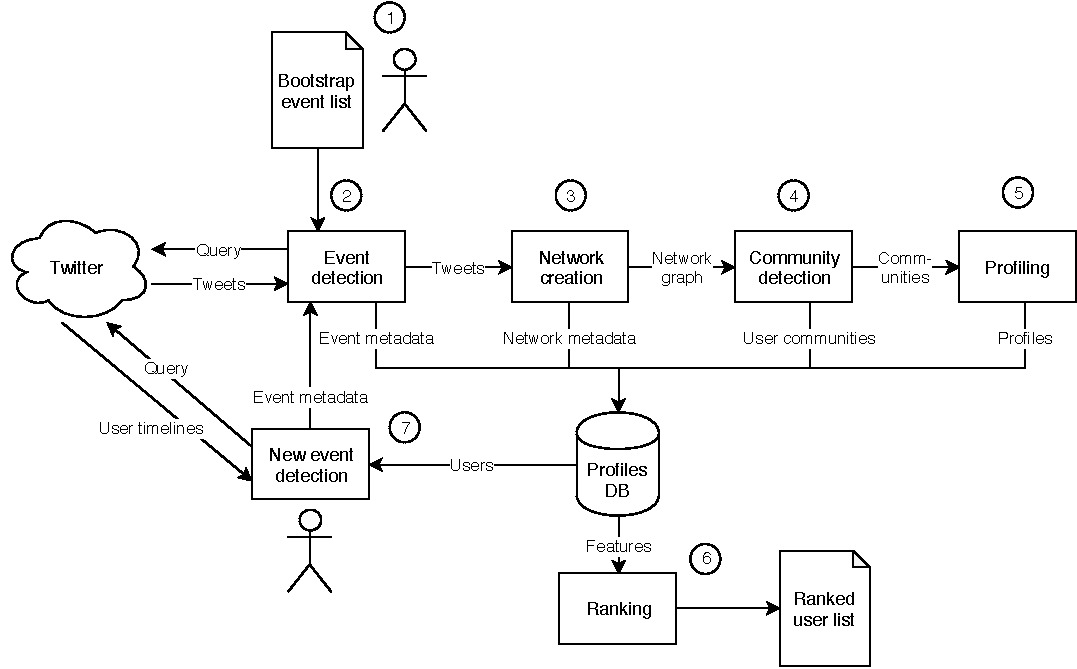
\includegraphics[width=0.7\linewidth]{figures/TwitterFramework}
	\caption{\comment{Schematic diagram of the user discovery framework }{this is a placeholder -- to be redrawn -PM }}
	\label{fig:twitterframework}
\end{figure*}

The iterative user discovery process is as follows.
Each iteration processes one context $C$. 

Firstly, all\footnote{Importantly, the Twitter API only allows a small fraction of the content history to be retrieved. We discuss this limitation in Sec. \ref{sec:limitations}.}
Twitter posts that satisfy the criteria set in $C$ are retrieved.

contexts are used to retrieve 
User interactions within the context are reconstructed using retweet and mention activities, and represented as a user-user network for each context. 
%
Context-independent follower/followee user relationships are also retrieved from Twitter and added to the network as additional user-user edges.
The size of the network is largely determined by the nature of the context, and may range from a few \hl{XX} users for a small context such as a local awareness event, to \hl{XX} users for a large national event that extends over a long timeframe, such as a political election campaign.

Large networks are further partitioned into communities, using the well-known Daemon community-detection algorithm \cite{DEMON}.
%
The goal of this further partitioning is to further narrow the scope and thus to enable weak-signal users to emerge relative to other influencers, who are socially more prominent but, in the context of our work, less interesting.
Relevance features are then computed for each user within the scope of each community. 
Finally, a relevance score is associated with each user in the context, and used to update their global score in the database of relevant users.

The final step in the iteration aims to discover new contexts. 
This is achieved by looking for relevant new keywords and hashtags and that are found in the post history (retrieved earlier) for the top-$k$ new users identified during the iteration. 
This last step is currently not automated, and involves humans who are knowledgeable with the domain. 
As such knowledge is not particularly deep or difficult to source, in the future we plan to crowdsource this particular step.

The new context constructed using the new keywords and hashtags are used to initiate the next iteration. 
While the process ends naturally when no new contexts are uncovered from the previous ones, the system continuously monitors the Twitter stream for recent contexts. These may typically include events that are temporally recurring, and use similar hashtags for each new edition. In this case, their relevance is assessed on the basis of their past history.


\subsection{Harvesting Content and Creating Context networks}  \label{sec:harvesting}

\anote{this is just a note on how data is collected from Twitter}

\subsection{Community detection}  \label{sec:communities}

\anote{describe Daemon in summary}

\subsection{User selection and ranking}  \label{sec:communities}

\anote{use network analysis for user selection. Mention in-degree centrality as the metric of choice, and justify intuitively (against others from the literature)}
\anote{remove white list users (manual step)}
\anote{user selection threshold as a parameter}

\anote{Then collect user content data for the top-k users, and compute their score using content metrics}
\anote{explain how each of the three families of metrics is computed -- when, what additional work is needed}

\subsection{New context discovery}  \label{sec:context-discovery}

\anote{as mentioned above, this is still manual so not much to say really?}

%\noindent Context $C$ $\rightarrow$ all users $U(C)$ \\
%$U(C)$ $\rightarrow$ retrieve context metrics $\rightarrow$ build context network $N(U(C))$ \\
%$N(U(C))$ $\rightarrow$ detect communities \\
%for each community: compute $\{ \mathit{in-degree}(u)\}_{u\in U}$ (relative to the community)\\
%
%in parallel also compute:\\
%- context-independent metrics\\
%- content-based metrics\\
%
%}

\section{Empirical Evaluation: activists} \label{sec:evaluation}



	
\section{Discussion and ongoing work}

\anote{
	we say that events are manually identified. Sketch the events bootstrapping idea.
}

 \bibliographystyle{splncs04}
 \bibliography{icwe19}

\end{document}
